\documentclass[oneside,a4paper,10pts,article]{memoir}
\usepackage[utf8]{inputenc}

\usepackage[danish]{isodate}

\usepackage{palatino}
\usepackage{graphicx}
\usepackage{todonotes}
\presetkeys{todonotes}{inline}{}

\usepackage{url}
\usepackage[hidelinks,hyperindex]{hyperref}

\captionnamefont{\bfseries}

\usepackage{tikz}
\usetikzlibrary{positioning,arrows,calc}

\newcommand{\vs}{%
    \tikz[remember picture,overlay]{\node at
        ($(current page.south east)+(-2,2)$)
        [anchor=south east] {Vend siden $\rightarrow$};}
}



\usepackage{listings}
\lstdefinelanguage{JavaScript}{
  keywords={break, case, catch, continue, debugger, default, delete,
    do, else, false, finally, for, function, if, in, instanceof, new,
    null, return, switch, this, throw, true, try, typeof, var, void,
    while, with},
  morecomment=[l]{//},
  morecomment=[s]{/*}{*/},
  morestring=[b]',
  morestring=[b]",
  ndkeywords={class, export, boolean, throw, implements, import, this},
  keywordstyle=\color{blue},
  ndkeywordstyle=\color{darkgray},
  identifierstyle=\color{black},
  commentstyle=\color{purple}\ttfamily,
  stringstyle=\color{red}\ttfamily,
  sensitive=true,
  extendedchars=true,
literate=%
{æ}{{\ae}}1
{å}{{\aa}}1
{ø}{{\o}}1
{Æ}{{\AE}}1
{Å}{{\AA}}1
{Ø}{{\O}}1
}

\lstset{
  basicstyle=\ttfamily\footnotesize,
  keywordstyle=\bfseries,
  captionpos=b,
  language=JavaScript
}

% Remove section numbers
\setsecnumdepth{part}

% Remove page numbers
\renewcommand\thepage{}

\title{Variable i Processing
  \\ {\normalfont\small\scshape Coding Pirates DIKU }} \date{\today}

\begin{document}
\maketitle
\vs
\chapter{Variable}
Tast det her ind:
\begin{lstlisting}
    var xpos = 200;
    rect(xpos, 50, 75, 75);
\end{lstlisting}
Prøv at ændre 200 til et andet tal.

\vspace{5mm}

\noindent
Eller prøv:
\begin{lstlisting}
    var diameter = 25;
    ellipse(200, 200, diameter, diameter);
\end{lstlisting}

\vspace{5mm}

\noindent
Fisk der kan bevæge sig:
\begin{lstlisting}
    var xpos = 200;
    ellipse(xpos, 200, 120, 75);
    triangle(xpos-60, 200, xpos-90, 170, xpos-90, 230);
\end{lstlisting}

\chapter{Opgaver}
\begin{itemize}
\item Farvelæg fisken
\item Giv fisken et øje
\item Lav en ny variabel til fisken, der styrer y-positionen
\item Få bilen fra sidste uge til at køre
\end{itemize}
\hspace{1cm}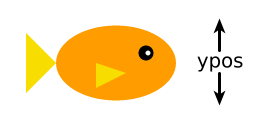
\includegraphics[width=0.4\textwidth]{pics/fisk-ypos.png}
\hspace{1cm}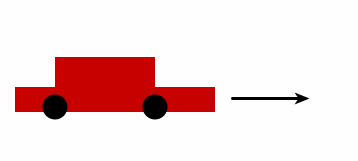
\includegraphics[width=0.5\textwidth]{pics/bil-frem.png}

\newpage
\chapter{Tegneprogram}

\noindent
Tegneprogram
\begin{lstlisting}
    fill(0, 0, 0);
    draw = function () {
      ellipse(mouseX, mouseY, 10, 10);
    };
\end{lstlisting}

\noindent
Slet alt med klik på musen:
\begin{lstlisting}
    mousePressed = function () {
      background(255, 255, 255);
    };
\end{lstlisting}

\chapter{Opgaver}

\begin{itemize}
\item Prøv at ændre tegneprogrammet til at bruge \texttt{line()}
\item Prøv at ændre farve vha. \texttt{mouseX/mouseY}
\item UFO der kan styres med musen

\hspace{1cm}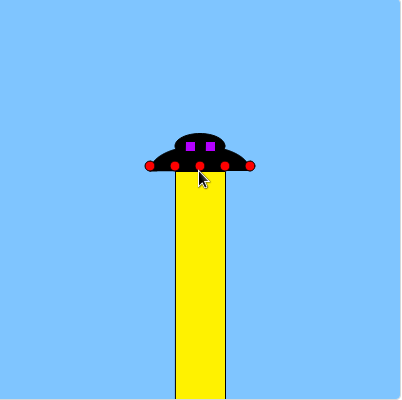
\includegraphics[width=0.4\textwidth]{pics/ufo.png}

\item 
Tegn streger fra hjørner til musen:

\hspace{1cm}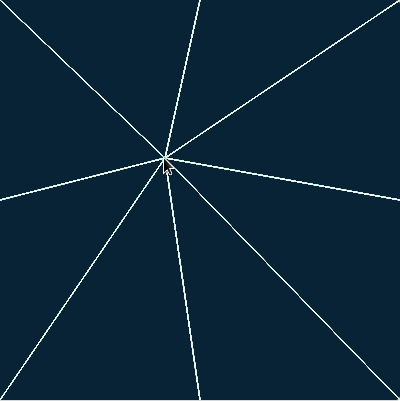
\includegraphics[width=0.4\textwidth]{pics/kryds.png}
\hspace{1cm}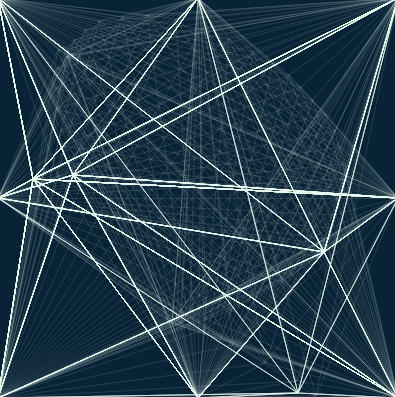
\includegraphics[width=0.4\textwidth]{pics/kryds-tegning.png}

Brug f.eks. farver:
\begin{lstlisting}
    background(9,35,54);
    stroke(233,249,247, 30);
\end{lstlisting}
Det fjerde argument til \texttt{stroke} er gennemsigtighed (0-100\%)!

\end{itemize}


\end{document}